\documentclass[10pt,aspectratio=43]{beamer}
\usetheme{Berlin}

\usepackage{amsmath,bm,amsfonts,amssymb,enumerate,graphicx,animate,epsfig,bbm,calc,color,ifthen,capt-of,multimedia}
\usepackage{fancybox,xcolor,booktabs,colortbl}
\usepackage{physics}
\usepackage{../mycommand}%我惯用的命令,在本project中,存储在本文件的父文件夹
\graphicspath{{figures/}}

\usefonttheme{professionalfonts}
\usepackage[UTF8,fontset=none,scheme=chinese]{ctex}
\setmainfont{Times}
\setsansfont{Arial}
\setmonofont{Consolas}
\setCJKmainfont{SimSun}[BoldFont=SimHei,ItalicFont=KaiTi]
\setCJKsansfont{SimHei}
\setCJKmonofont{Microsoft YaHei}
\usepackage{unicode-math}
\setmathfont{XITS Math}

\usepackage{../beamercolorthemesustech}%效果同\usecolortheme{sustech},但\usecolortheme不支持自由选择文件路径,故调用底层的\usepackage命令
\definecolor{mygreen}{rgb}{0,0.6,0}
\definecolor{mymauve}{rgb}{0.58,0,0.82}
\definecolor{mygray}{gray}{.9}
\definecolor{mypink}{rgb}{.99,.91,.95}
\definecolor{mycyan}{cmyk}{.3,0,0,0}

\usepackage[ruled,linesnumbered]{algorithm2e}
\usepackage{verbatim,listings}
\lstset{ %
	backgroundcolor=\color{white},   % choose the background color
	basicstyle=\footnotesize\ttfamily,     % size of fonts used for the code
	columns=fullflexible,
	breaklines=true,                 % automatic line breaking only at whitespace
	captionpos=b,                    % sets the caption-position to bottom
	tabsize=4,
	commentstyle=\color{mygreen},    % comment style
	escapeinside={\%*}{*)},          % if you want to add LaTeX within your code
	keywordstyle=\color{blue},       % keyword style
	stringstyle=\color{mymauve}\ttfamily,     % string literal style
	numbers=left, 
	%	frame=single,
	rulesepcolor=\color{red!20!green!20!blue!20},
	% identifierstyle=\color{red},
	language=c
}

\setbeamertemplate{caption}[numbered]%添加图片的编号
\setbeamertemplate{sidebar right}{}%去掉默认添加的navigarion symbols
\setbeamercovered{transparent}%使未点出来的文字呈现透明,默认0.15透明度
\beamerdefaultoverlayspecification{}

%\usepackage[backend=biber,bibstyle=gb7714-2015,citestyle=verbose]{biblatex}
%\addbibresource{../reference.bib}

%题目,作者,学校,日期
\title{Boundedness and Stability}
\subtitle{\fontsize{9pt}{14pt}\textbf{第五次\quad SDEM 5.4}}
\author{杨徵羽}
%\institute{哈尔滨工业大学(威海)理学院}
\date{\today}

\begin{document}

\frame{\titlepage}

\begin{frame}{全章结构}
\begin{table}[htbp]%\caption{全章结构}\label{t1}\centering
\resizebox{\columnwidth}{!}{
\begin{tabular}{cccccc}
\toprule
稳定性种类 & 节 & 定义 & V函数判别法 & 系数判别法 & 例子 \\
\midrule
p阶矩渐近有界 & 5.2 & 1 & 2 & 3 & 4,5 \\
p阶矩指数稳定 & 5.3 & 7 & 8 & 10,12,16 & 25,26,27 \\
p阶矩渐近稳定 & 5.4 & 28 & 29,30,31 &  & 32,33 \\
a.s.指数稳定 & 5.3 & 7 & 9 & 10,12,13,14,16 &  \\
a.s.渐近稳定 & 5.4 & 28 & 29 &  &  \\
依概率稳定 & 5.5 & 34 & 35 &  &  \\
依概率渐近稳定 & 5.5 & 34 & 36 &  & 38 \\
依概率渐近大范围稳定 & 5.5 & 34 & 37 &  &  \\
依分布渐近稳定 & 5.6 & 40 & 43 & 44 & 45,46 \\
\bottomrule
\end{tabular}
}
\end{table}
\end{frame}

\begin{frame}{Theorem 5.24(部分思路)}
\setcounter{equation}{0}
\fontsize{7.5}{0}\selectfont
\begin{align}
&\mathbb{E}|x(t\wedge\tau_z)|^p=\mathbb{E}\Bigg(\xi(t\wedge\tau_z)\prod_{k=0}^{n-1}\zeta_k\Bigg)=\mathbb{E}\Bigg(\bigg(\xi(t\wedge\tau_z)\prod_{k=0}^{n-2}\zeta_k\bigg)\zeta_{k-1}\Bigg)\\
={}&\mathbb{E}\Bigg(\bigg(\xi(t\wedge\tau_z)\prod_{k=0}^{n-2}\zeta_k\bigg)\mathbb{E}(\zeta_{k-1}|\mathcal{G})\Bigg)\\
={}&\mathbb{E}\Bigg(\bigg(\xi(t\wedge\tau_z)\prod_{k=0}^{n-2}\zeta_k\bigg)\sum_{i\in\mathbb{S}}I_{\{r(t\wedge\tau_z)=i\}}\mathbb{E}(\zeta_{k-1}(i)|\mathcal{G})\Bigg)\\
={}&\mathbb{E}\Bigg(\bigg(\xi(t\wedge\tau_z)\prod_{k=0}^{n-2}\zeta_k\bigg)\sum_{i\in\mathbb{S}}I_{\{r(t\wedge\tau_z)=i\}}\mathbb{E}\zeta_{k-1}(i)\Bigg)\\
={}&\mathbb{E}\Bigg(\bigg(\xi(t\wedge\tau_z)\prod_{k=0}^{n-2}\zeta_k\bigg)\sum_{i\in\mathbb{S}}I_{\{r(t\wedge\tau_z)=i\}}\Bigg)\\
={}&\mathbb{E}\Bigg(\xi(t\wedge\tau_z)\prod_{k=0}^{n-2}\zeta_k\Bigg)\\
={}&\cdots=\mathbb{E}\xi(t\wedge\tau_z)
\end{align}
\fontsize{10}{0}\selectfont
\end{frame}

\begin{frame}{5.4 Asymptotic Stability}
\begin{itemize}
\item Definition 5.28: p阶矩/a.s.渐近稳定性定义
\item Theorem 5.29: p阶矩/a.s.渐近稳定性V函数判别法(Step 1:与Theorem 5.9类似的估计方法;Step 2:区间放缩,积分转化为级数;Step 3:类似控制收敛下的求和积分换序)
\item Theorems 5.30,31: p阶矩渐近稳定性V函数判别法的两个推广(反证法,$ L^p $估计,$ \mathcal{K},\Psi $类函数性质,Jensen不等式)
\item Examples 5.32,33: 数值算例
\end{itemize}
\end{frame}

\begin{frame}{Theorem 5.29}
\setcounter{equation}{0}
\begin{align}
&\text{已知条件}\notag\\
→{}&\int_{0}^{\infty}\mathbb{E}|x(t)|^p\mathrm{d}t<\infty\\
→{}&\int_{0}^{\infty}\mathbb{E}\sup_{t\le s\le t+\delta}|x(s)|^p\mathrm{d}t<\infty\\
→{}&\sum_{k=1}^{\infty}\mathbb{E}\sup_{\frac{k\delta}{2}\le s\le \frac{(k+1)\delta}{2}+\delta}|x(s)|^p<\infty\\
→{}&\mathbb{E}\sum_{k=1}^{\infty}\sup_{\frac{k\delta}{2}\le s\le \frac{(k+1)\delta}{2}+\delta}|x(s)|^p<\infty
\end{align}
\end{frame}

\begin{frame}{Theorem 5.30}
\setcounter{equation}{0}
\begin{align}
&\text{已知条件}\notag\\
→{}&\mathbb{E}|x(t)|^p<K\\
→{}&|\mathbb{E}|x(t)|^p-\mathbb{E}|x(s)|^p|\le C(t-s)\\
→{}&\lim_{t\to\infty}\mathbb{E}|x(t)|^p=0
\end{align}
\end{frame}

\begin{frame}{上上上上次的$ LV $计算(SDEM p.159)}
\begin{figure}
\centering
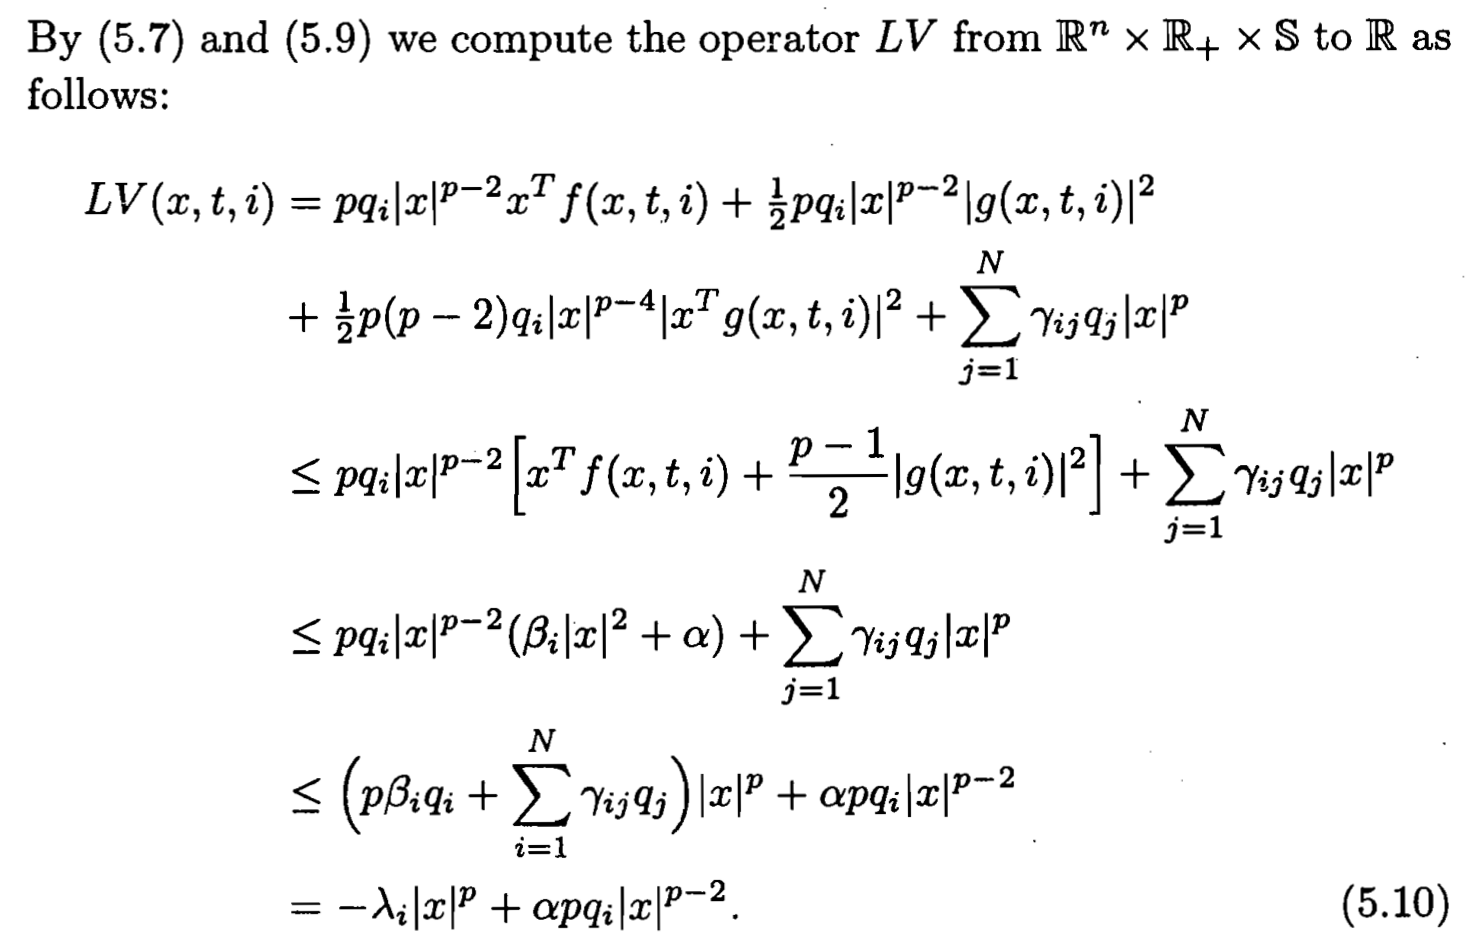
\includegraphics[width=\linewidth]{1}
\end{figure}
\end{frame}

\begin{frame}{BDG不等式(SDE p.127)}
\begin{figure}
\centering
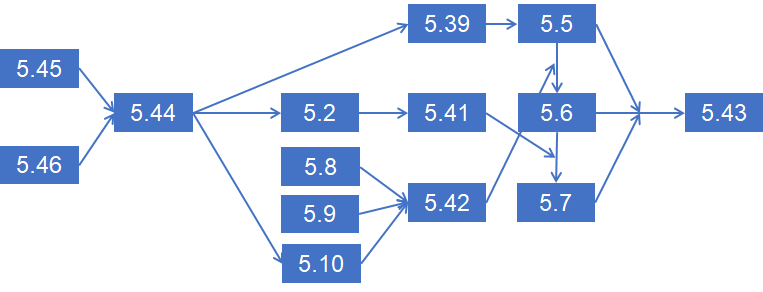
\includegraphics[width=\linewidth]{2}
\end{figure}
\end{frame}

\end{document}
